% =========================================================================
\documentclass[notes, aspectratio=1610]{beamer}
%\documentclass[aspectratio=1610]{beamer}

% ========================= Theme =========================================
\usetheme{Berkeley}
\usecolortheme{seahorse}

% ========================= Essential packages ============================
%\usepackage{hyperref}
%\hypersetup{
%    colorlinks = true,
%    linkcolor = blue,
%    citecolor = blue,
%    filecolor = blue,
%    urlcolor = blue
%}

% ========================= Frame notes systm ============================
%\usepackage{pgfpages}
%\setbeameroption{show notes on second screen}

% ========================= Plotting ======================================
\usepackage{calc}
\usepackage{tikz}
\usetikzlibrary{arrows,
                arrows.meta,
                calc,
		chains,
                quotes,
                positioning,
		shapes,
                shapes.geometric}
\usepackage{graphicx}
\usepackage{graphics}
\usepackage{pgfplots}
\pgfplotsset{width=7cm,compat=1.17}

%% ============================== Tabular =================================
\usepackage{booktabs}
\usepackage{tabularx,ragged2e}
\usepackage{array}
\usepackage{multirow}
\usepackage{siunitx}
  \sisetup{detect-all}
\usepackage{adjustbox}
\usepackage{rotating}
\usepackage{threeparttable}
\usepackage[justification=centering]{caption}
\usepackage{color, colortbl}

%% ============================== Text boxes ==============================
\usepackage[most]{tcolorbox}		

% ========================= Infor on authors ==============================
%\title[Visualization Design]%
%{Visualization Design}
\title{Timelines and Narratives}
\author{S.~Santoni\inst{1}\inst{2}}
\institute{
	\inst{1}%
	Bayes Business School
	\and
	\inst{2}%
	Soundcloud
	}
\date{MSc in Business Analytics, 2022/23}

% ============================ Colors =====================================
\definecolor{base_c}{rgb}{0.6,0,0}
\definecolor{comp_c}{rgb}{0.09803921568627451, 0.6901960784313725, 0.7529411764705882}
\definecolor{tri_1}{rgb}{0.09803921568627451, 0.7686274509803922, 0.19215686274509805}
\definecolor{tri_2}{rgb}{0.19215686274509805, 0.09803921568627451, 0.7686274509803922}

% ========================= TOC  ==========================================
\AtBeginSection[]
{
	\begin{frame}
		       \frametitle{Outline}
		       \tableofcontents[currentsection,currentsubsection]
	\end{frame}
}

% ========================= References ===================================
\usepackage[style=numeric,backend=biber]{biblatex}
\addbibresource{bibliography.bib}

% ========================= Document  ====================================
\begin{document}

\begin{frame}
	\titlepage
\end{frame}

\begin{frame}{Outline}
	\tableofcontents
\end{frame}

% ========================== Temporal Data Viz ===========================
\section{The Nuts and Bolts of Temporal Data Viz}

\begin{frame}{Ice-Breaker Question}{}
	\centering 
	\Large 
	How does `time' matter for data visualization?
\end{frame}

\begin{frame}{How Does `Time' Matter for Data Visualization?}
	{Example 1: Napoleon's Russian Campaign}
	\centering 
	\Large

	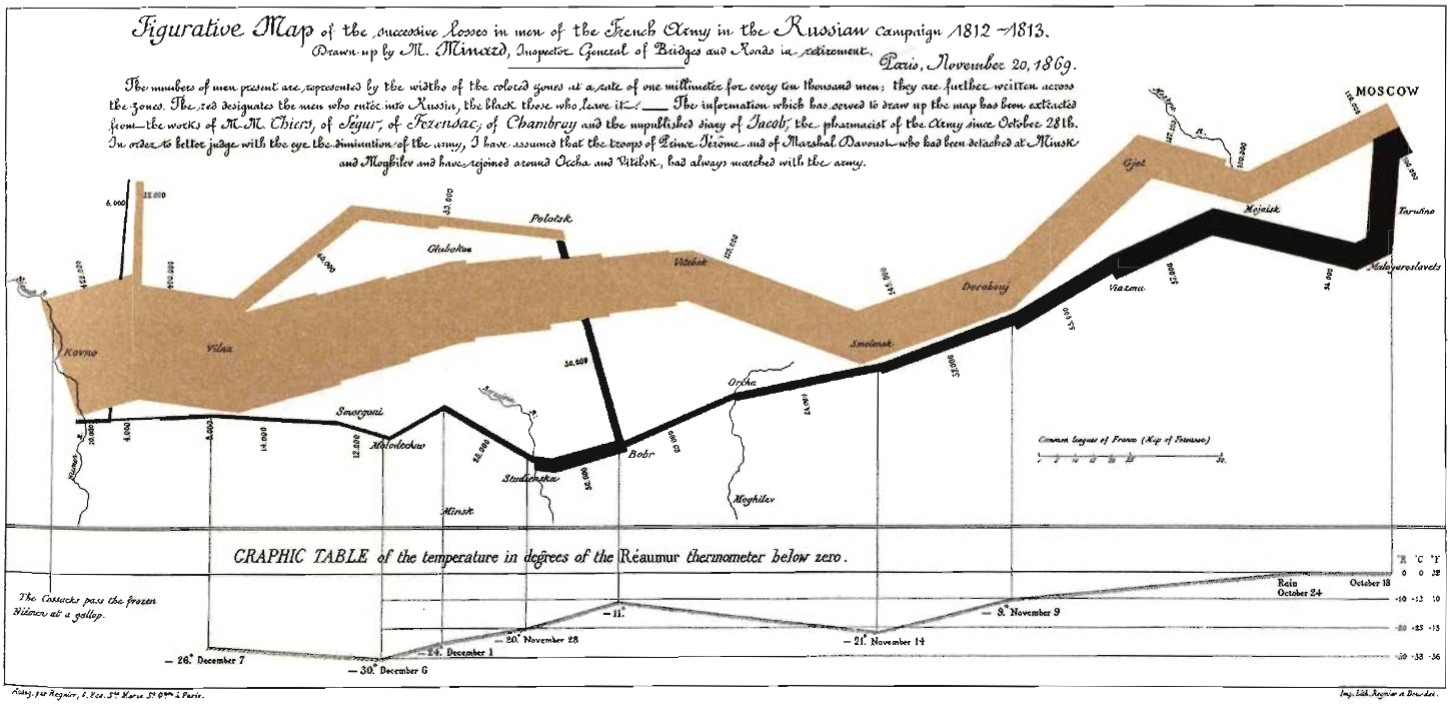
\includegraphics[width=0.9\textwidth]{images/russian_campaign.png}

\end{frame}

\begin{frame}{How Does `Time' Matter for Data Visualization?}
	{Example 1: Napoleon's Russian Campaign}
	\centering 
	\Large

	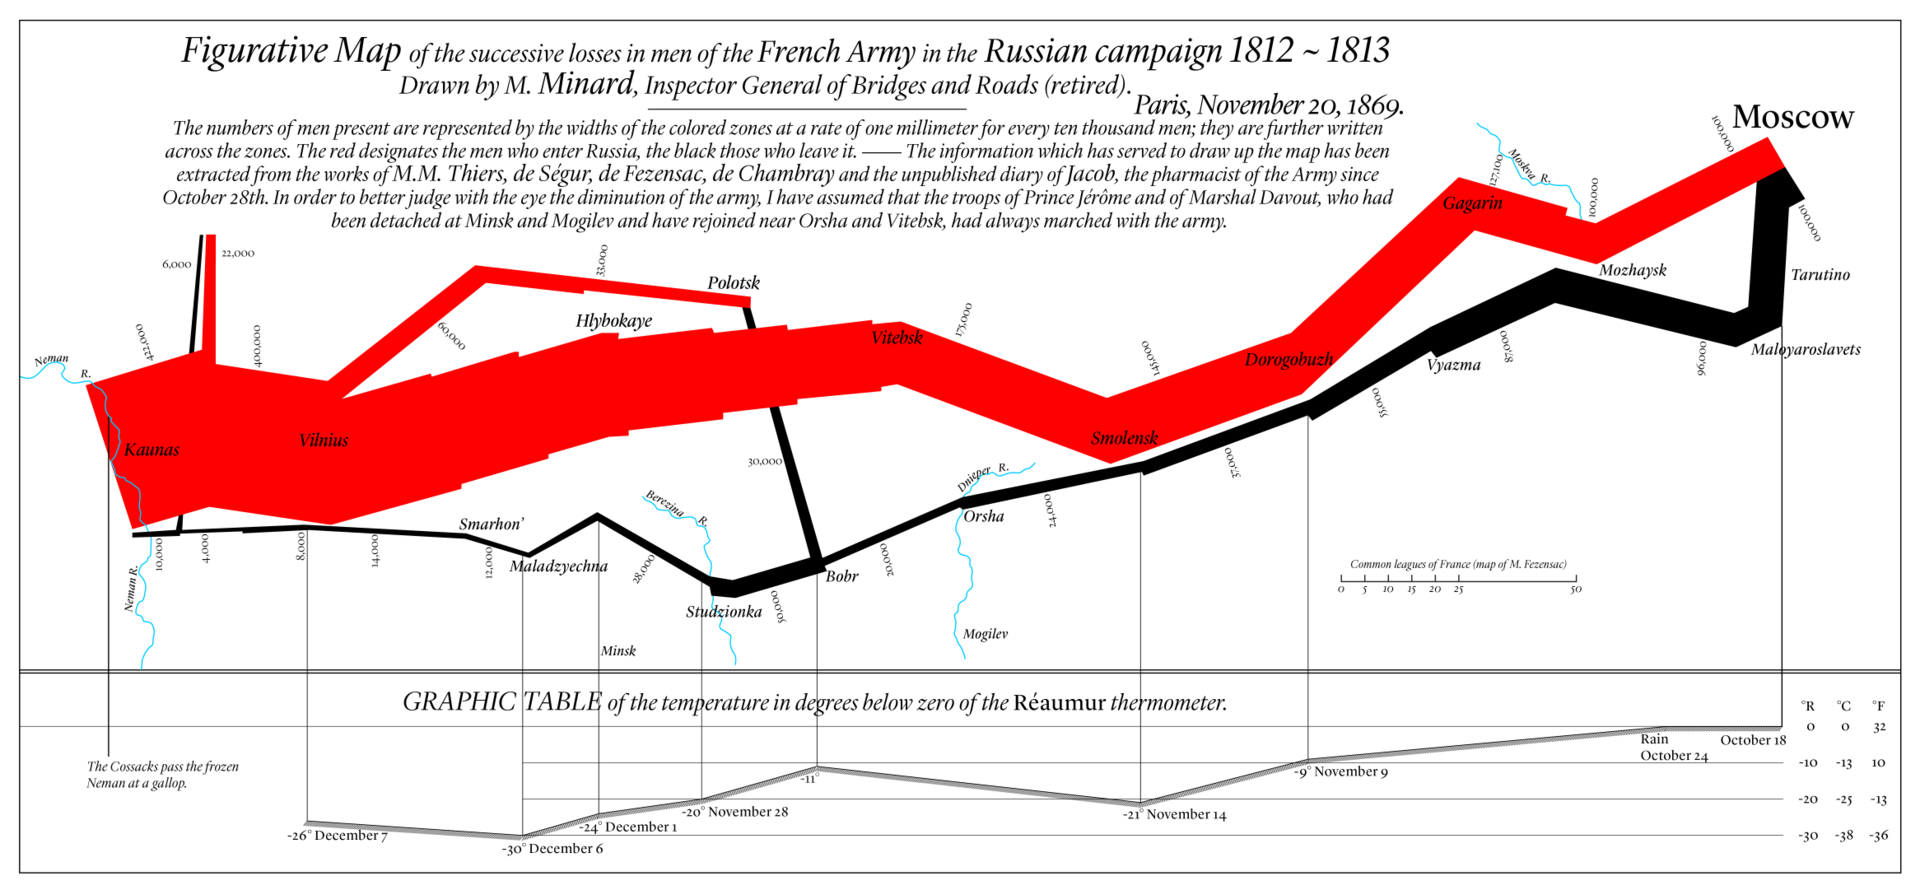
\includegraphics[width=0.9\textwidth]{images/1920px-Minard_Update.png}

\end{frame}


\begin{frame}{How Does `Time' Matter for Data Visualization?}
	{Example 2: strong openers and late bloomers}
	\centering 
	\Large 

	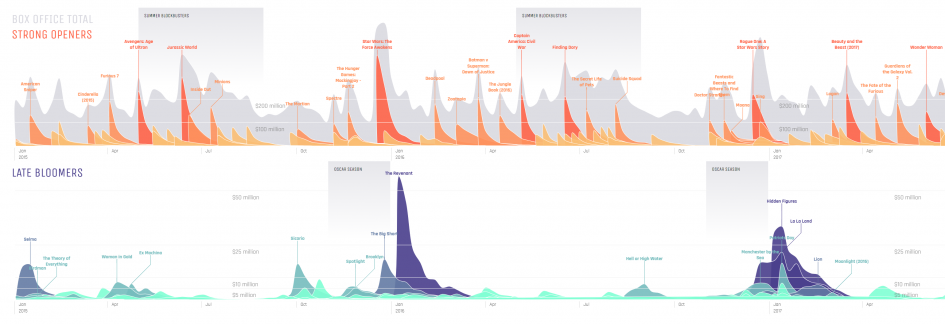
\includegraphics[width=0.9\textwidth]{images/Day57-945x324.png}

\end{frame}

\begin{frame}{Time-Related Viz: Goals}{}
Provided our data include a temporal dimension, we may want to show one of 
the following 

\begin{itemize}
	\item 
	Change in a continuous variable
	\item 
	Change in a qualitative (i.e., categorical) variable
	\item 
	Sequences of change --- i.e., patterns of change in a continuous or
	qualitative variable
	\item 
	Connections among events
\end{itemize}

\end{frame}

\begin{frame}{Time-Related Viz: Analytical Approaches}{}

There are two possible analytical approaches to investigating/visualize 
data with a temporal dimension:

\begin{itemize}
	\item 
	Within-case approach
	\item 
	Comparative, within- \& between-case approach
\end{itemize}
 
\end{frame}

\begin{frame}{Time-Related Viz: Analytical Approaches}
	{A single time series is suited to the within-case approach}

	\centering

	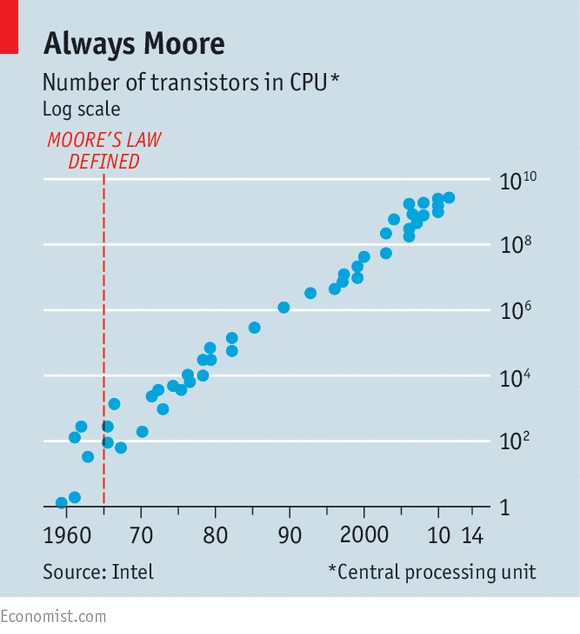
\includegraphics[width=0.5\textwidth]{images/20150418_WBC823_0.png}

\end{frame}

\begin{frame}{Time-Related Viz: Analytical Approaches}
	{A multiple time-series/panel is suited to the within- \& 
	between-case approach}

	\centering

	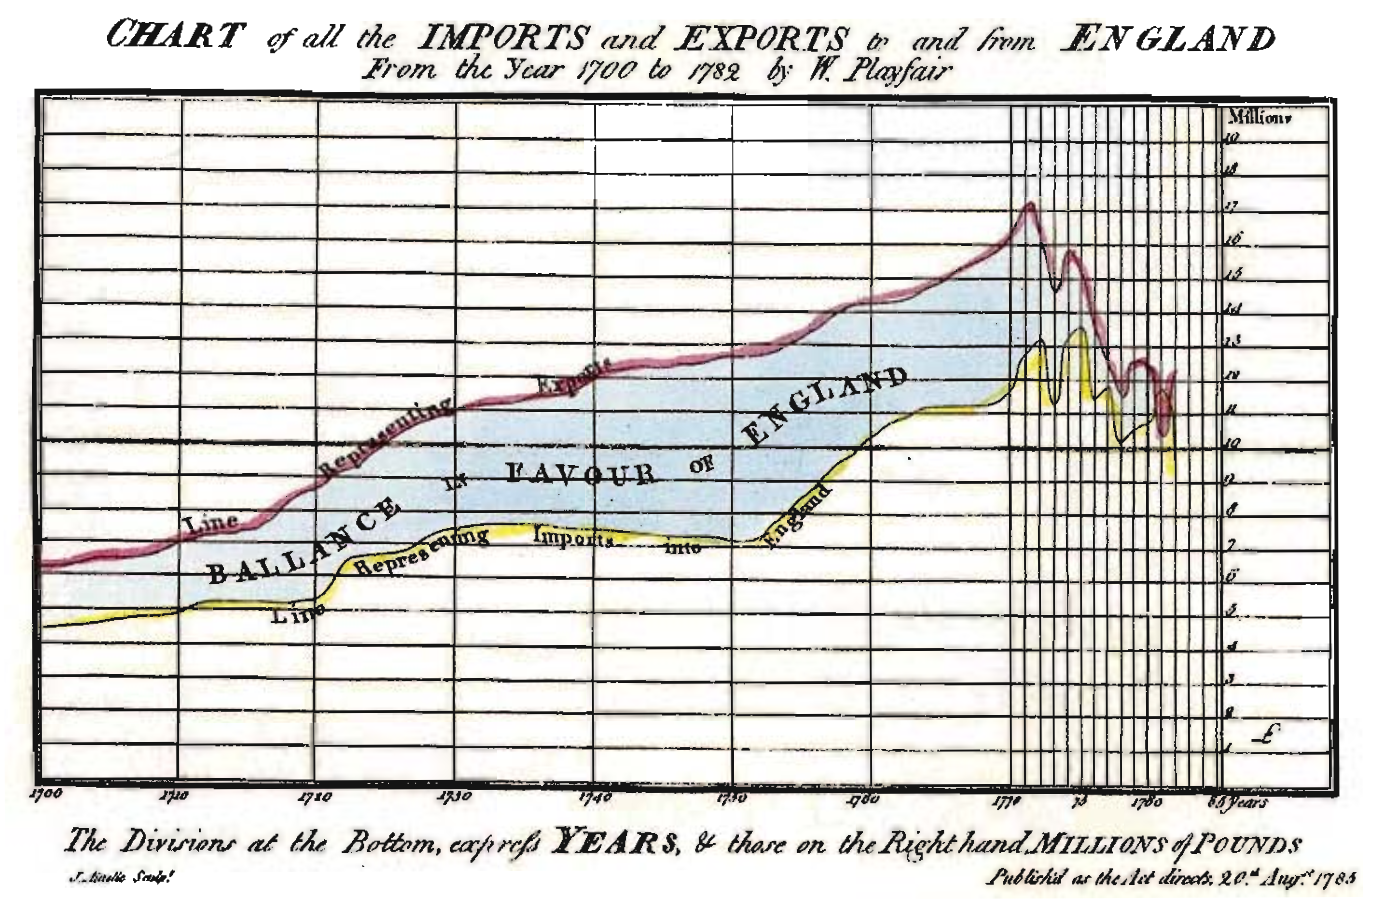
\includegraphics[width=0.8\textwidth]{images/import_export.png}

\end{frame}

%% =========================== exemplars ==================================
\section{Exemplars of Temporal Data Viz}

\begin{frame}{Popularity of YouTube Videos}
	{Miotto, José M., and Eduardo G. Altmann. ``Predictability of extreme 
	events in social media.'' PloS one 9, no. 11 (2014): e111506.}
	\centering

	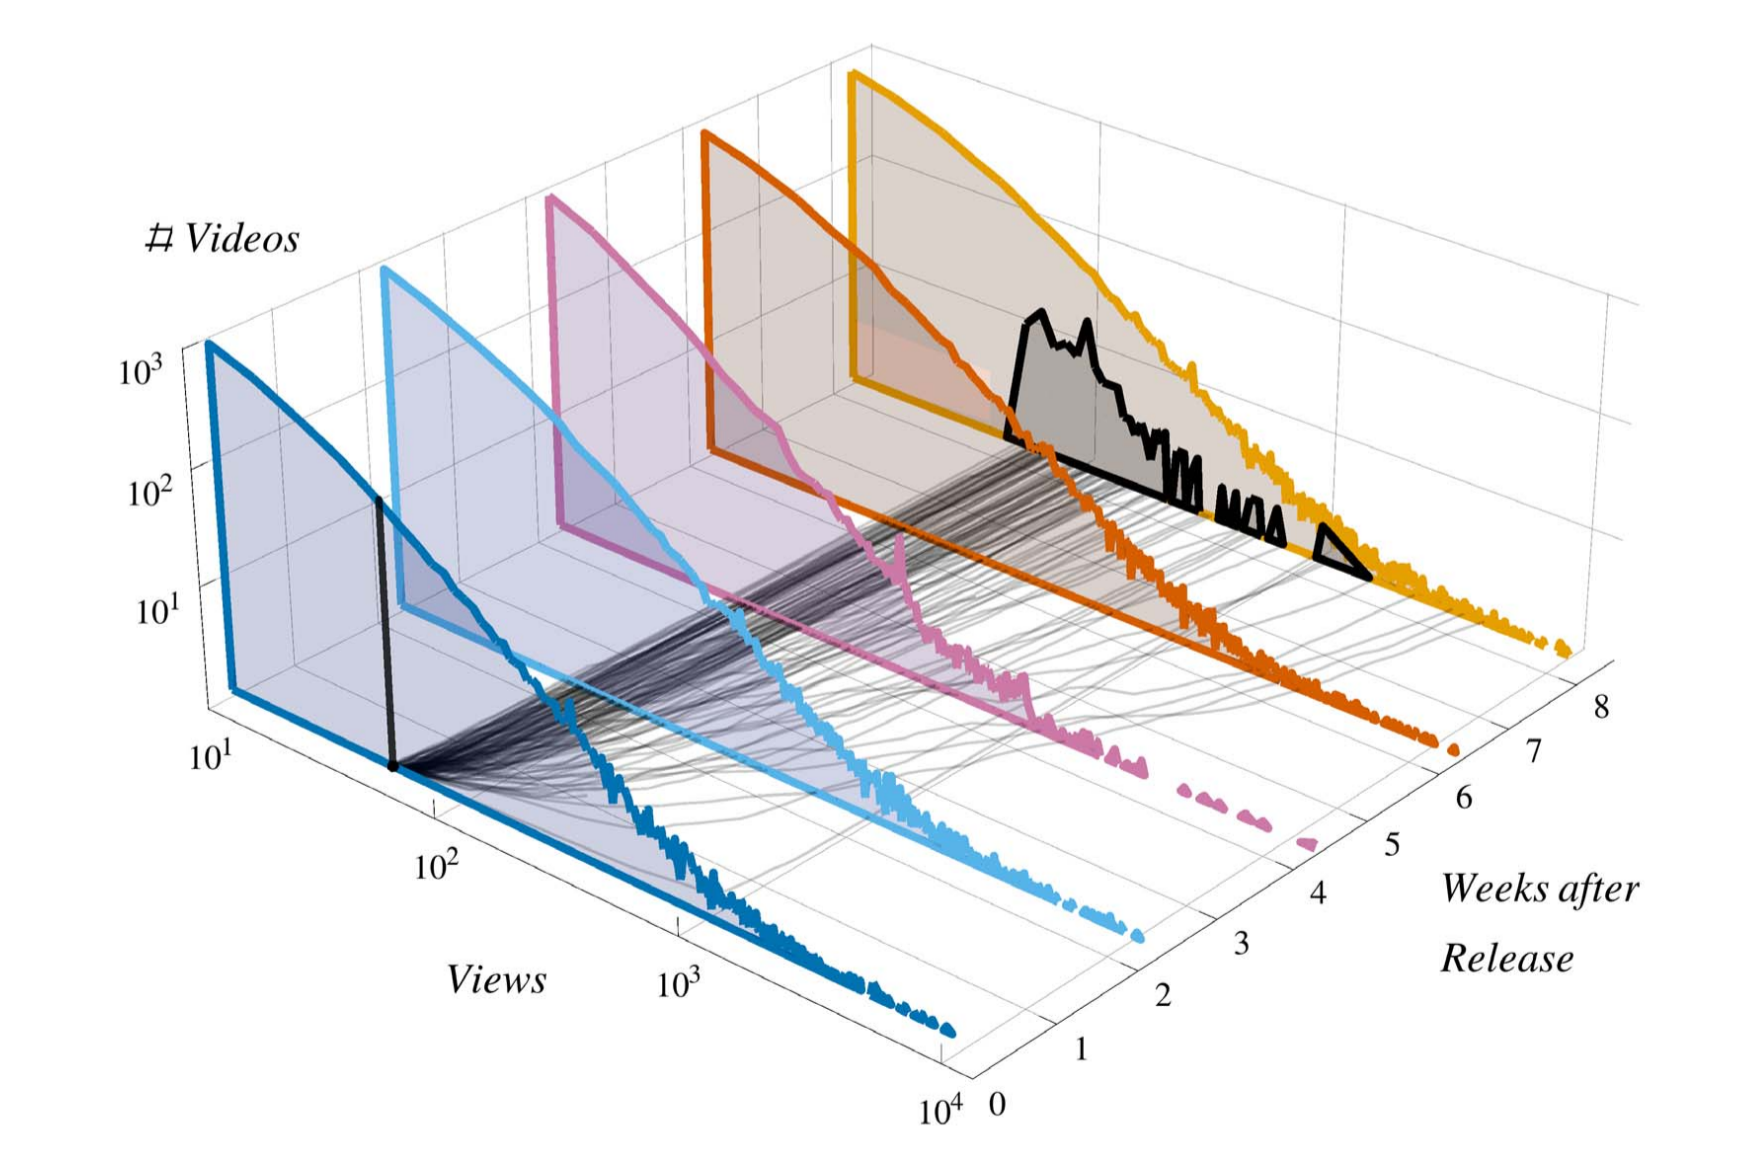
\includegraphics[width=0.8\textwidth]{images/youtube_popularity.png}
\end{frame}

\begin{frame}{US Senate Voting Similarity Over Time}
	{Source: Moody, James, and Peter J. Mucha. ``Portrait of political 
	party polarization1.'' Network Science 1, no. 1 (2013): 119-121.}
	\centering

	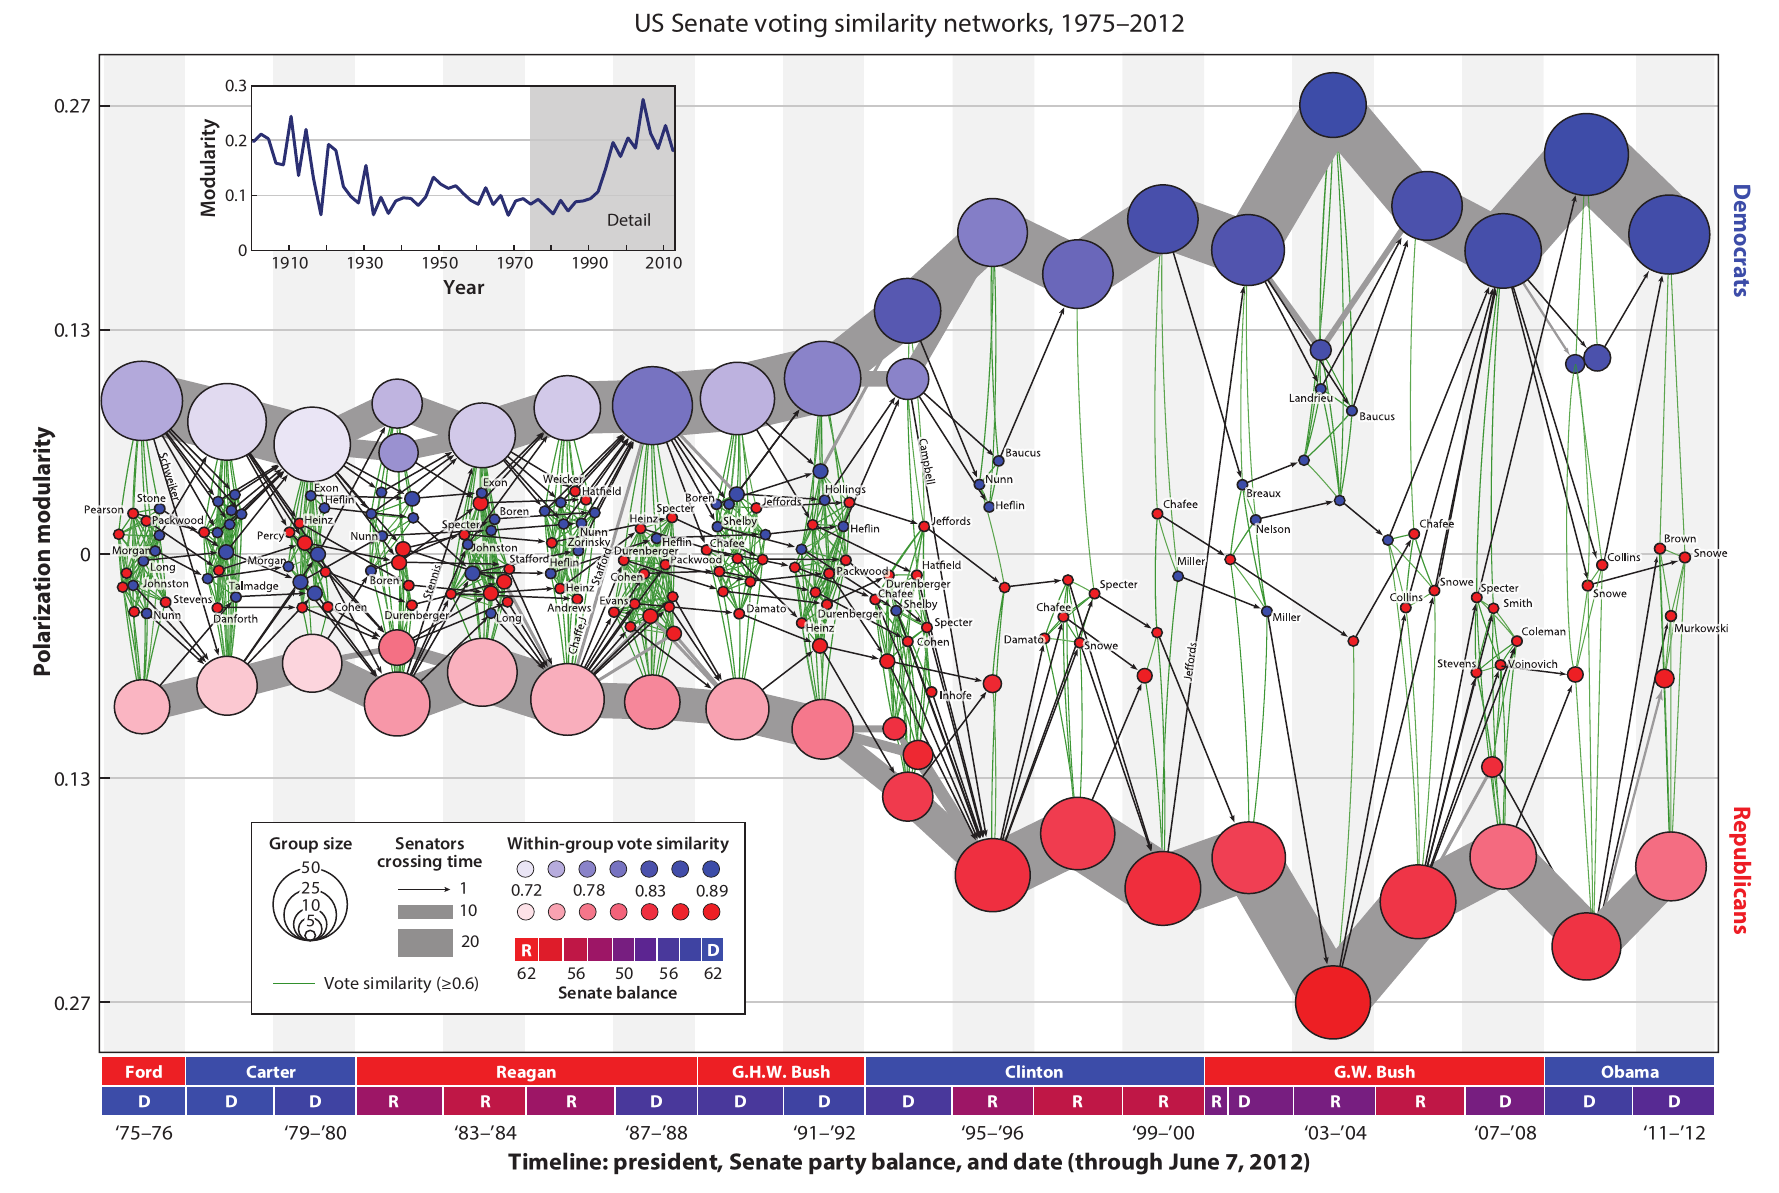
\includegraphics[width=0.85\textwidth]{images/moody_mucha.png}
\end{frame}

%% =========================== Lab =========================================

\section{Handling Time-Related Data with Pandas}

\begin{frame}{Let Us Go Back to the SMM692 Notes}{}
	\centering 

	
\includegraphics[width=0.5\textwidth]{images/smm692_notes}
\end{frame}

% =========================== Bibliography =================================
%\begin{frame}
%	\frametitle{References}
%	\printbibliography
%\end{frame}

% =========================== Close ========================================
\end{document}